\section{Gui\-Engine Class Reference}
\label{classGuiEngine}\index{GuiEngine@{GuiEngine}}
{\tt \#include $<$gui\-Engine.hpp$>$}

Collaboration diagram for Gui\-Engine:\begin{figure}[H]
\begin{center}
\leavevmode
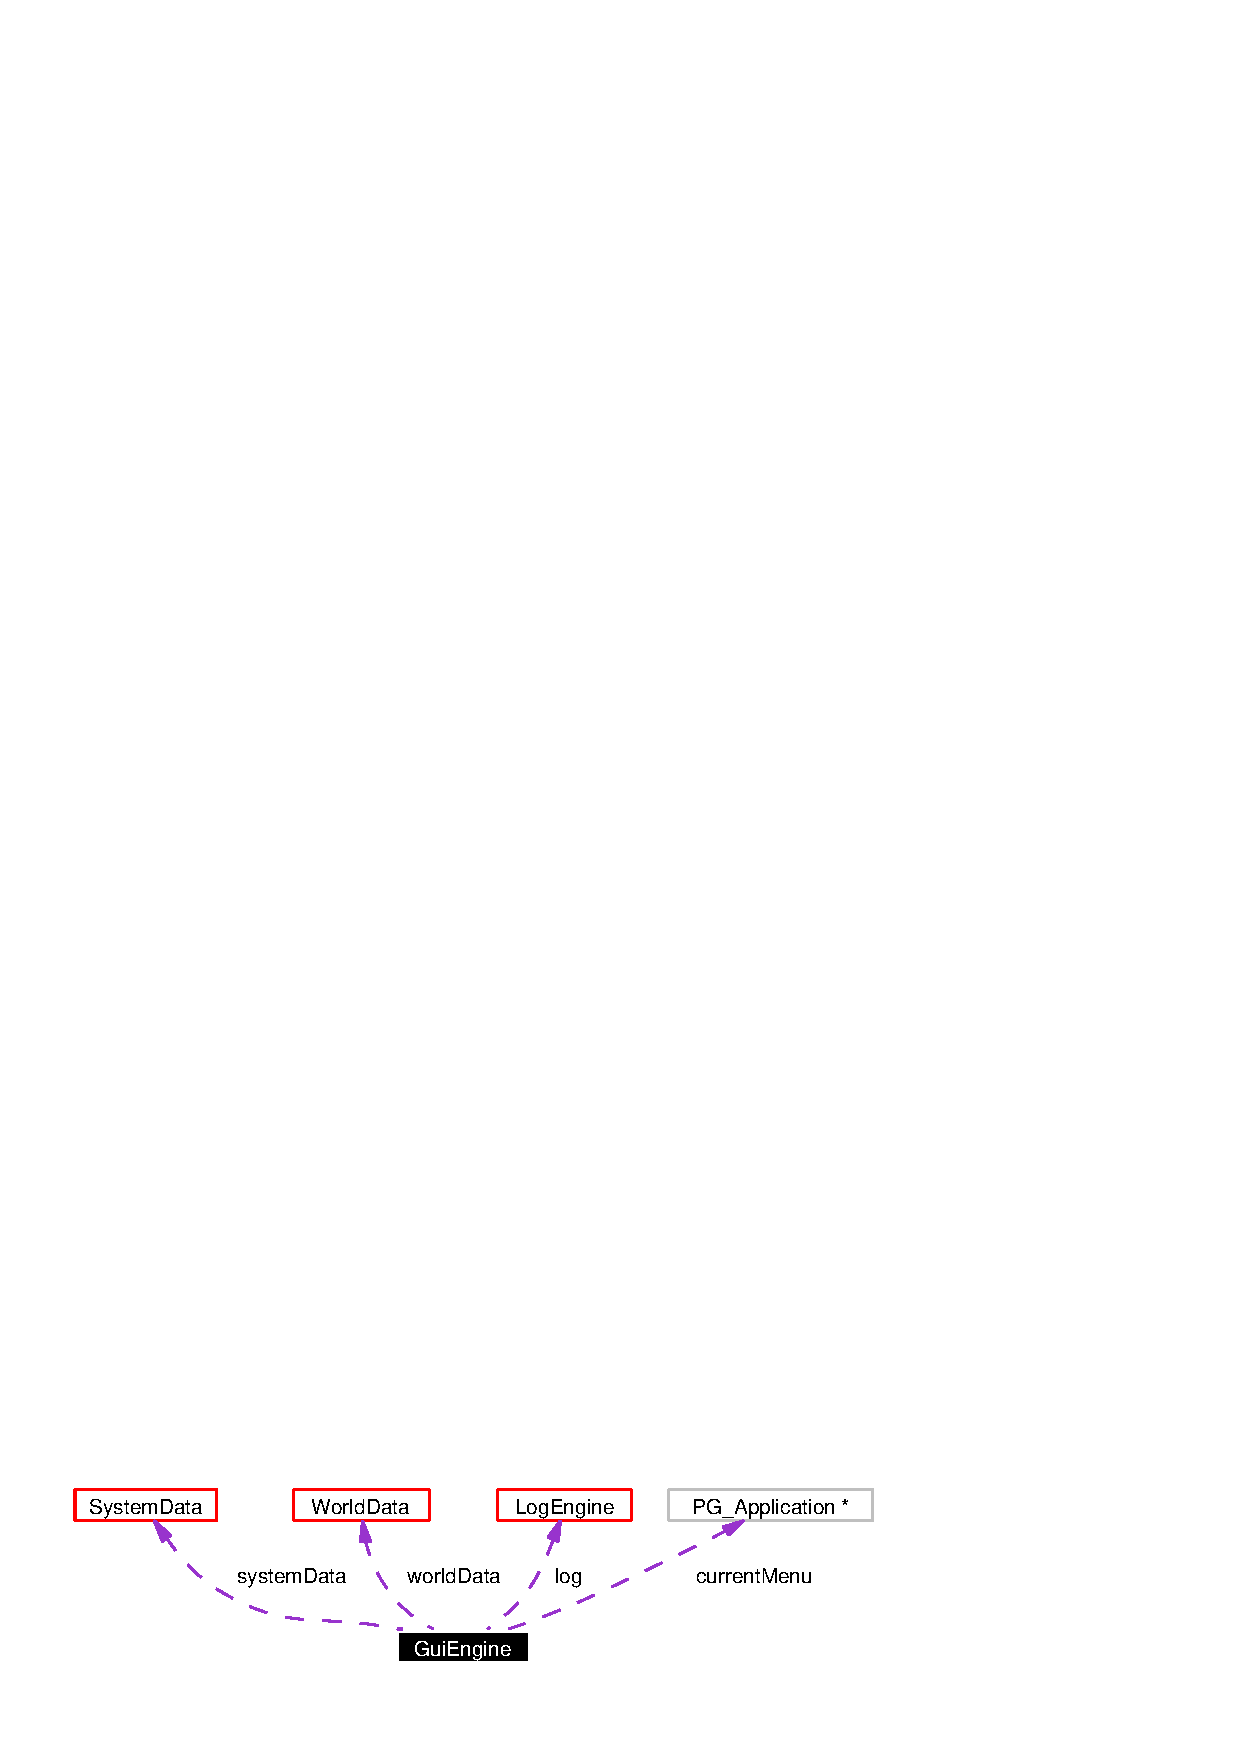
\includegraphics[width=223pt]{classGuiEngine__coll__graph}
\end{center}
\end{figure}
\subsection*{Public Member Functions}
\begin{CompactItemize}
\item 
int {\bf options\-Menu} (void)
\item 
int {\bf main\-Menu} (void)
\item 
int {\bf test\-Basic\-Paragui} (void)
\item 
int {\bf start} ({\bf World\-Data} $\ast$wrl\-Data, {\bf System\-Data} $\ast$sys\-Data)
\item 
int {\bf step} (void)
\item 
int {\bf stop} (void)
\item 
PG\_\-Application $\ast$ {\bf get\-Current\-Menu} (void)
\item 
{\bf World\-Data} $\ast$ {\bf get\-World\-Data} (void)
\item 
{\bf System\-Data} $\ast$ {\bf get\-System\-Data} (void)
\item 
{\bf Log\-Engine} $\ast$ {\bf get\-Log} (void)
\end{CompactItemize}
\subsection*{Private Attributes}
\begin{CompactItemize}
\item 
{\bf Log\-Engine} {\bf log}
\item 
{\bf World\-Data} $\ast$ {\bf world\-Data}
\item 
{\bf System\-Data} $\ast$ {\bf system\-Data}
\item 
PG\_\-Application $\ast$ {\bf current\-Menu}
\end{CompactItemize}


\subsection{Member Function Documentation}
\index{GuiEngine@{Gui\-Engine}!getCurrentMenu@{getCurrentMenu}}
\index{getCurrentMenu@{getCurrentMenu}!GuiEngine@{Gui\-Engine}}
\subsubsection{\setlength{\rightskip}{0pt plus 5cm}PG\_\-Application $\ast$ Gui\-Engine::get\-Current\-Menu (void)}\label{classGuiEngine_a6}


\index{GuiEngine@{Gui\-Engine}!getLog@{getLog}}
\index{getLog@{getLog}!GuiEngine@{Gui\-Engine}}
\subsubsection{\setlength{\rightskip}{0pt plus 5cm}{\bf Log\-Engine} $\ast$ Gui\-Engine::get\-Log (void)}\label{classGuiEngine_a9}


\index{GuiEngine@{Gui\-Engine}!getSystemData@{getSystemData}}
\index{getSystemData@{getSystemData}!GuiEngine@{Gui\-Engine}}
\subsubsection{\setlength{\rightskip}{0pt plus 5cm}{\bf System\-Data} $\ast$ Gui\-Engine::get\-System\-Data (void)}\label{classGuiEngine_a8}


\index{GuiEngine@{Gui\-Engine}!getWorldData@{getWorldData}}
\index{getWorldData@{getWorldData}!GuiEngine@{Gui\-Engine}}
\subsubsection{\setlength{\rightskip}{0pt plus 5cm}{\bf World\-Data} $\ast$ Gui\-Engine::get\-World\-Data (void)}\label{classGuiEngine_a7}


\index{GuiEngine@{Gui\-Engine}!mainMenu@{mainMenu}}
\index{mainMenu@{mainMenu}!GuiEngine@{Gui\-Engine}}
\subsubsection{\setlength{\rightskip}{0pt plus 5cm}int Gui\-Engine::main\-Menu (void)}\label{classGuiEngine_a1}


\index{GuiEngine@{Gui\-Engine}!optionsMenu@{optionsMenu}}
\index{optionsMenu@{optionsMenu}!GuiEngine@{Gui\-Engine}}
\subsubsection{\setlength{\rightskip}{0pt plus 5cm}int Gui\-Engine::options\-Menu (void)}\label{classGuiEngine_a0}


\index{GuiEngine@{Gui\-Engine}!start@{start}}
\index{start@{start}!GuiEngine@{Gui\-Engine}}
\subsubsection{\setlength{\rightskip}{0pt plus 5cm}int Gui\-Engine::start ({\bf World\-Data} $\ast$ {\em wrl\-Data}, {\bf System\-Data} $\ast$ {\em sys\-Data})}\label{classGuiEngine_a3}


\index{GuiEngine@{Gui\-Engine}!step@{step}}
\index{step@{step}!GuiEngine@{Gui\-Engine}}
\subsubsection{\setlength{\rightskip}{0pt plus 5cm}int Gui\-Engine::step (void)}\label{classGuiEngine_a4}


\index{GuiEngine@{Gui\-Engine}!stop@{stop}}
\index{stop@{stop}!GuiEngine@{Gui\-Engine}}
\subsubsection{\setlength{\rightskip}{0pt plus 5cm}int Gui\-Engine::stop (void)}\label{classGuiEngine_a5}


\index{GuiEngine@{Gui\-Engine}!testBasicParagui@{testBasicParagui}}
\index{testBasicParagui@{testBasicParagui}!GuiEngine@{Gui\-Engine}}
\subsubsection{\setlength{\rightskip}{0pt plus 5cm}int Gui\-Engine::test\-Basic\-Paragui (void)}\label{classGuiEngine_a2}




\subsection{Member Data Documentation}
\index{GuiEngine@{Gui\-Engine}!currentMenu@{currentMenu}}
\index{currentMenu@{currentMenu}!GuiEngine@{Gui\-Engine}}
\subsubsection{\setlength{\rightskip}{0pt plus 5cm}PG\_\-Application$\ast$ {\bf Gui\-Engine::current\-Menu}\hspace{0.3cm}{\tt  [private]}}\label{classGuiEngine_r3}


\index{GuiEngine@{Gui\-Engine}!log@{log}}
\index{log@{log}!GuiEngine@{Gui\-Engine}}
\subsubsection{\setlength{\rightskip}{0pt plus 5cm}{\bf Log\-Engine} {\bf Gui\-Engine::log}\hspace{0.3cm}{\tt  [private]}}\label{classGuiEngine_r0}


\index{GuiEngine@{Gui\-Engine}!systemData@{systemData}}
\index{systemData@{systemData}!GuiEngine@{Gui\-Engine}}
\subsubsection{\setlength{\rightskip}{0pt plus 5cm}{\bf System\-Data}$\ast$ {\bf Gui\-Engine::system\-Data}\hspace{0.3cm}{\tt  [private]}}\label{classGuiEngine_r2}


\index{GuiEngine@{Gui\-Engine}!worldData@{worldData}}
\index{worldData@{worldData}!GuiEngine@{Gui\-Engine}}
\subsubsection{\setlength{\rightskip}{0pt plus 5cm}{\bf World\-Data}$\ast$ {\bf Gui\-Engine::world\-Data}\hspace{0.3cm}{\tt  [private]}}\label{classGuiEngine_r1}




The documentation for this class was generated from the following files:\begin{CompactItemize}
\item 
src/gui/{\bf gui\-Engine.hpp}\item 
src/gui/{\bf gui\-Engine.cpp}\end{CompactItemize}
